\chapter{神经网络量子态}\label{chap:neural_network_quantum_state}
\section{循环神经网络波函数}
循环神经网络(recurrent neural network, RNN)是一类用于处理序列数据的神经网络,其具有自回归性(autoregressive property):
条件概率$P(\sigma_n | \sigma_{<n})$仅取决于$\sigma_{1},\cdots,\sigma_{n-1}$。因此常用来预测前后相关的变量模型,在语言建模、机器翻译、语音识别等场景应用广泛。

相较于玻尔兹曼机,用自回归神经网络表示量子态的优势主要在于其高效、准确的采样能力。用玻尔兹曼机表示量子态时,为了优化参数以及计算物理量期望值,往往要采用马尔科夫链蒙特卡罗(Markov chain Monte Carlo)采样的方法,从引导波函数中采样。
然而这种方式在问题规模大、目标函数势能图景复杂的情况下,一方面往往带来很高的计算成本,另一方面也很难避免得到真正独立、没有关联的样本。这在一定程度上阻碍了神经网络的表示能力,使得优化过程变得低效。
而自回归神经网络在采样时,依照条件概率对各个变量进行依次采样,因此准确、高效,便于并行化。得到的样本彼此之间独立,没有关联,可以更好地发挥神经网络的表示能力。

% 近几年来,有不少自回归神经网络结合变分原理描述经典、量子系统平衡系统的成功尝试:
% $P(\boldsymbol{\sigma})=P(\sigma_1)P(\sigma_2 |\sigma_1)\cdots P(\sigma_N | \sigma_{N-1}, \cdots, \sigma_2, \sigma_1)$,
% 即
\subsection{循环神经网络(RNN)}
我们采用循环神经网络模拟一个未知的概率分布。假定该概率分布中每一个变量组态$\boldsymbol{\sigma}\equiv (\sigma_{1}, \sigma_{2}, \cdots, \sigma_{N})$包含$N$个二进制变量$\sigma_n \in \{0,1\}$。

我们采用$P(\boldsymbol{\sigma})\equiv P(\sigma_{1}, \sigma_{2}, \cdots, \sigma_{N})$表示一个变量组态对应的概率。由于循环神经网络的自回归性,有:
\begin{equation} \label{eq:rnn_autoregressive}
    \adddotsbeforeeqnnum%
    P(\boldsymbol{\sigma})=P(\sigma_1)P(\sigma_{2}|\sigma_1)\cdots P(\sigma_{N} | \sigma_{N-1}, \cdots, \sigma_{2}, \sigma_1)
\end{equation}

其中$P(\sigma_{i}|\sigma_{i-1}, \cdots,\sigma_{2},\sigma_1)\equiv P(\sigma_i | \sigma_{<i})$是给定所有$j<i$变量$\sigma_j$下$\sigma_i$的条件概率。
当所有条件概率$P(\sigma_i | \sigma_{<i})$都确定时,变量组态$\boldsymbol{\sigma}$对应的概率$P(\boldsymbol{\sigma})$也就确定了。

\begin{figure}[!htbp]
    \centering
    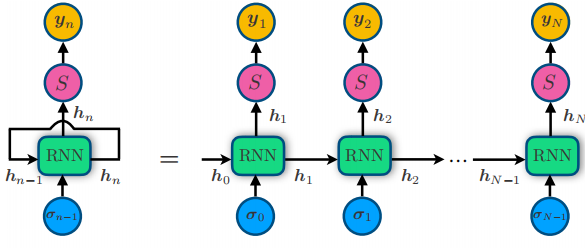
\includegraphics[width=0.60\textwidth]{rnn}
    \bicaption{循环神经网络}{Recurrent Neural Network}
    \label{fig:rnn}
\end{figure}

RNN的基本构建模块是一个循环单元,如图~\ref{fig:rnn}所示,最简单的循环单元是一个非线性函数,该函数将$d_h$维隐藏矢量$\boldsymbol{h}_{n-1}$和二维输入矢量$\boldsymbol{\sigma}_{n-1}$映射为$d_h$维输出隐藏矢量$\boldsymbol{h}_n$。
即:
\begin{equation} \label{eq:rnn_h_n}
    \adddotsbeforeeqnnum%
    \boldsymbol{h}_{n} = f(W[\boldsymbol{h}_{n-1};\boldsymbol{\sigma}_{n-1}]+\boldsymbol{b})
\end{equation}

其中$f$是非线性激活函数,例如sigmoid函数、双曲正切函数、ELU函数等等。$\boldsymbol{W}\in \mathbb{R}^{d_{h}\times (d_{h}+2)}$是权重矩阵。$\boldsymbol{b}\in \mathbb{R}^{d_h}$是偏差矢量。
$[\boldsymbol{a};\boldsymbol{b}]$表示向量$\boldsymbol{a}$和$\boldsymbol{b}$的直和。
为起始循环,需要选定$\boldsymbol{h}_0$和$\boldsymbol{\sigma}_0$的值。$\boldsymbol{\sigma}_n$是输入$\sigma_n$的独热编码,即每个$\sigma_n$的值对应$\boldsymbol{\sigma}$的一位。
由于我们所关心的问题中,变量都是二进制的,因此$\sigma_{n}=0$对应$\boldsymbol{\sigma}=(1,0)$,$\sigma_{n}=1$对应$\boldsymbol{\sigma}=(0,1)$。

变量组态$\boldsymbol{\sigma}$对应的概率$P(\boldsymbol{\sigma})$可以通过循序地计算条件概率得到:
\begin{equation} \label{eq:rnn_P}
    \adddotsbeforeeqnnum%
    P(\sigma_{n}|\sigma_{n-1},\cdots,\sigma_1)=\boldsymbol{y}_{n}\cdot \boldsymbol{\sigma}_n
\end{equation}

其中$\boldsymbol{y}_n=(y_{n}^{1},y_{n}^{2})$是一个二维矢量,其分量是正实数,所有分量之和等于1。$\boldsymbol{y}_{n}$由下式定义:
\begin{equation} \label{eq:rnn_y_n}
    \adddotsbeforeeqnnum%
    \boldsymbol{y}_n \equiv S\left(U \boldsymbol{h}_n+\boldsymbol{c}\right)
\end{equation}

其中$U\in \mathbb{R}^{2\times d_{h}}$是Softmax层的权重项,$c\in \mathbb{R}^{2}$是偏差项。Softmax激活函数$S$为:
\begin{equation} \label{eq:softmax}
    \adddotsbeforeeqnnum%
    S(v_{n})=\frac{\text{exp}(v_n)}{\sum_{i}\text{exp}(v_i)}
\end{equation}

由式~\eqref{eq:rnn_autoregressive}和式~\eqref{eq:rnn_P}可知,变量组态$\boldsymbol{\sigma}$对应的概率$P(\boldsymbol{\sigma})$为:
\begin{equation}
    \adddotsbeforeeqnnum%
    P(\boldsymbol{\sigma})=\prod_{n=1}^{N}\boldsymbol{y}_{n}\cdot \boldsymbol{\sigma}_n
\end{equation}

由$\boldsymbol{y}_n$分量之和等于1的性质可知,$\sum_{\boldsymbol{\sigma}}P(\boldsymbol{\sigma})=1$,因此用RNN表示的概率分布是归一的。

对RNN进行采样时,同样根据条件概率分布,循序地确定$\boldsymbol{h}_1, \boldsymbol{y}_1$,然后根据$\boldsymbol{y}_1$确定$\sigma_1$的值,以此类推,直到$\boldsymbol{\sigma}=(\sigma_{1}, \sigma_{2}, \cdots, \sigma_{N})$完全确定。

实际应用时,由于RNN在捕捉变量间的长程关联时可能会导致梯度爆炸或消失,因此常采用更加复杂的改进结构。